\subsection{Attore Insegnante} 
\subsubsection{UC-1 Inserimento esercizio}
\begin{figure}[htbp]
	\centering
	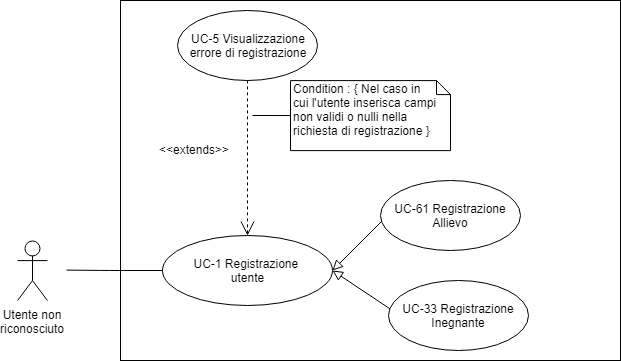
\includegraphics[scale=0.7]{images/UC-1.png}
	\caption{UC-1 Inserimento esercizio}
\end{figure}
	\begin{itemize}
		\item \textbf{Attori: } Insegnante
		\item \textbf{Descrizione scenario: } L'utente si è loggato come insegnante e ha scelto di inserire un nuovo esercizio. Per fare ciò deve fornire un nome dell'esercizio. Dovrà essere inserita una frase, la richiesta dell'esercizio è compiere l'analisi grammaticale di questa frase. È richiesto l'inserimento di un livello di difficoltà dell'esercizio. L'utente potrà inoltre scegliere se assegnare l'esercizio a qualche sua classe di allievi.
Infine l'esercizio potrà essere salvato.
		\item \textbf{Precondizione: }L'utente si è loggato come insegnante ed ha scelto di inserire un nuovo esercizio.
		\item \textbf{Flusso degli eventi: }
		\begin{itemize}
		\item UC-1.1 Inserire il nome dell'esercizio
		\item UC-1.2 Inserire la frase dell'esercizio
		\item UC-1.3 Inserire la soluzione dell'esercizio
		\item UC-1.4 Inserire un livello di difficoltà
		\item UC-1.5 Assegnare l'esercizio a zero o una o più classi
		\item UC-1.6 Scelta esercizio pubblico o privato
		\item UC-1.7 Salvare le esercizio
		\end{itemize}
		\item \textbf{Estensioni: }
		\begin{itemize}
		\item UC-1.1.1 Nel caso in cui il nome inserito sia già esistente tra gli esercizi creati.
		\item UC-1.2.1 La frase potrebbe essere già presente nella piattaforma.
		\item UC-1.3.1 Se la frase fosse già presente nella piattaforma, durante la fase di inserimento della soluzione l'utente potrà scegliere di utilizzare la soluzione della frase già esistente, altrimenti verrà proposta una soluzione generata automaticamente.
		\item UC-1.7.1 I campi compilati potrebbero presentare errori, magari anche già segnalati ma ignorati. In questo caso il salvataggio non verrà eseguito e un messaggio d'errore segnalerà all'utente di ricontrollare i campi non validi.
		\end{itemize}
		\item \textbf{Postcondizione: }Il sistema salverà l'esercizio, esso verrà aggiunto alla lista degli esercizi creati dall'insegnante
	\end{itemize}
\subsubsection{UC-1.1 Inserimento nome esercizio}
\begin{itemize}
\item \textbf{Attori: }Insegnante
\item \textbf{Descrizione scenario: }L'insegnante volendo inserire un nuovo esercizio, deve inserire un nome per tale esercizio.
\item \textbf{Precondizione: }Insegnante ha scelto di inserire un nuovo esercizio e il sistema attende che l'utente inserisca un nome per questo esercizio
\item \textbf{Postcondizione: }La casella contenente il nome dell'esercizio che l'utente vuole inserire è compilata, e se il nome inserito risulterà corretto in fase di salvataggio non verranno riscontrati problemi.
\end{itemize}
\subsubsection{UC-1.1.1 Errore nome già esistente}
\begin{itemize}
\item \textbf{Attori: }Insegnante
\item \textbf{Descrizione scenario: }L'insegnante volendo inserire un nuovo esercizio, deve inserire un nome per tale esercizio, ma questo nome è già presente tra gli esrcizi creati dall'insegnante.
\item \textbf{Precondizione: }Insegnante ha inserito un nome per l'esercizio, ma il nome risultà essere già presente tra gli esrcizi creati dall'insegnante.
\item \textbf{Postcondizione: }Verrà mostrato un messaggio d'errore che riferirà all'utente di modificare il nome inserito.
\end{itemize}
\subsubsection{UC-1.2 Inserimento frase}
\begin{itemize}
\item \textbf{Attori: }Insegnante
\item \textbf{Descrizione scenario: }L'insegnante volendo inserire un nuovo esercizio, deve inserire una frase per tale esercizio.
\item \textbf{Precondizione: }L'insegnante ha scelto di inserire un nuovo esercizio e il sistema attende che l'utente inserisca una frase per questo esercizio.
\item \textbf{Postcondizione: }La casella per l'inserimento della frase dell'esercizio è compilata, e se la frase inserita risulterà valida in fase di salvataggio non verranno riscontrati problemi.
\end{itemize}
\subsubsection{UC-1.2.1 Frase già esistente}
\begin{itemize}
\item \textbf{Attori: }Insegnante
\item \textbf{Descrizione scenario: }L'insegnante volendo inserire un nuovo esercizio, deve inserire una frase per tale esercizio e questa risulta essere già esistente in altri esercizi pubblicati nella piattaforma.
\item \textbf{Precondizione: }L'insegnante ha inserito una frase per questo esercizio e la frase è oggetto di altri esercizi pubblicati nella piattaforma.
\item \textbf{Postcondizione: }Verrà mostrato un messaggio per notificare l'evento all'utente.
\end{itemize}
\subsubsection{UC-1.3 Inserimento soluzione}
\begin{figure}[htbp]
	\centering
	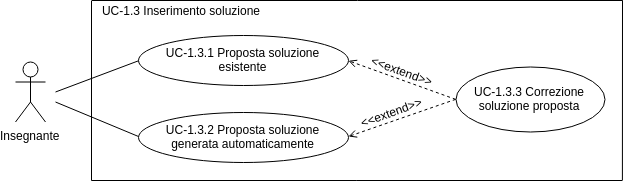
\includegraphics[scale=0.7]{images/UC-1_3.png}
	\caption{UC-1.3 Inserimento soluzione}
\end{figure}
\begin{itemize}
\item \textbf{Attori: }Insegnante
\item \textbf{Descrizione scenario: }L'insegnante ha inserito una frase dell'esercizio, deve inserire una soluzione per tale frase. Nel caso la frase inserita esista già in un esercizio pubblicato nella piattaforma l'utente può scegliere la soluzione già esistente di tale esercizio, oppure può scegliere una soluzione generata automaticamente. Nel caso la frase inserita non esista già nel sistema l'utente potrà utilizzare unicamente la proposta di soluzione generata automaticamente.
\item \textbf{Precondizione: }L'insegnante ha inserito una frase, ora può scegliere tra una proposta di soluzione esistente e una proposta di soluzione generata automaticamente, nel caso la frase inserita sia già esistente nel sistema. Altrimenti verrà proposta la soluzione generata automaticamente.
		\item \textbf{Flusso degli eventi: }
		\begin{itemize}
		\item UC-1.3.1 Proposta soluzione esistente, se la frase inserita esiste già.
		\item UC-1.3.2 Proposta soluzione generata automaticamente
		\item UC-1.3.3 Correzzione soluzione proposta
		\end{itemize}
\item \textbf{Estensioni: }
		\begin{itemize}
		\item UC-1.3.3 L'utente potrà correggere la soluzione proposta se questa non dovesse soddisfarlo.
		\end{itemize}
\item \textbf{Postcondizione: }L'utente ha scelto tra la soluzione già esistente e quella generata automaticamente. Il sistema può procedere con la proposta di soluzione per la frase inserita.
\end{itemize}
\subsubsection{UC-1.3.1 Proposta soluzione esistente}
\begin{itemize}
\item \textbf{Attori: }Insegnante
\item \textbf{Descrizione scenario: }L'insegnante ha inserito una frase già esistente in altri esercizi pubblicati nella piattaforma, ed ha scelto di compilare la soluzione del suo esercizio partendo dalla soluzione già esistente nella piattaforma. Potrà poi eventualmente modificare la soluzione proposta a suo piacimento.
\item \textbf{Precondizione: }L'insegnante ha inserito una frase già esistente in altri esercizi pubblicati nella piattaforma, ed ha scelto di compilare la soluzione del suo esercizio partendo dalla soluzione già esistente nella piattaforma.
\item \textbf{Postcondizione: }La soluzione per la frase inserita è stata compilata.
\end{itemize}
\subsubsection{UC-1.3.2 Proposta soluzione generata automaticamente}
\begin{itemize}
\item \textbf{Attori: }Insegnante
\item \textbf{Descrizione scenario: }L'insegnante ha inserito una frase già esistente in altri esercizi pubblicati nella piattaforma, ed ha scelto di compilare la soluzione del suo esercizio partendo dalla soluzione generata automaticamente. Potrà poi eventualmente modificare la soluzione proposta a suo piacimento.
\item \textbf{Precondizione: }L'insegnante ha inserito una frase già esistente in altri esercizi pubblicati nella piattaforma, ed ha scelto di compilare la soluzione del suo esercizio partendo dalla generata automaticamente.
\item \textbf{Postcondizione: }La soluzione per la frase inserita è stata compilata.
\end{itemize}
\subsubsection{UC-1.3.3 Correzione soluzione proposta}
\begin{itemize}
\item \textbf{Attori: }Insegnante
\item \textbf{Descrizione scenario: }Sia nel caso venga scelta una soluzione già esistente che nel caso venga usata una soluzione generata l'utente può correggere eventuali errori delle soluzioni proposte. Dopo aver osservato la soluzione proposta ha scelto di modificare qualche aspetto della soluzione, quindi di correggerla.
\item \textbf{Precondizione: }L'insegnante dopo aver osservato la soluzione proposta ha scelto di correggerla.
\item \textbf{Postcondizione: }La soluzione per la frase inserita è stata corretta e risulta essere compilata.
\end{itemize}
\subsubsection{UC-1.4 Inserimento livello di difficoltà}
\begin{itemize}
\item \textbf{Attori: }Insegnante
\item \textbf{Descrizione scenario: }L'utente sta inserendo un nuovo esercizio, e la piattaforma richiede l'inserimento di un livello di difficoltà dell'esercizio, in base alla qunatità delle diverse tipologie di parole presenti nella frase.
\item \textbf{Precondizione: }L'insegnante deve inserire un livello di difficoltà dell'esercizio.
\item \textbf{Postcondizione: }Il livello di difficoltà dell'esercizio è stato inserito.
\end{itemize}
\subsubsection{UC-1.5 Assegnazione esercizio a zero o più classi}
\begin{itemize}
\item \textbf{Attori: }Insegnante
\item \textbf{Descrizione scenario: }L'utente sta inserendo un nuovo esercizio, se l'utente possiede delle classi di allievi registrate nella piattaforma allora può scegliere se assegnare l'esercizio che sta inserendo qualcuna tra queste classi.
\item \textbf{Precondizione: }L'insegnante ha delle classi di allievi registrate nel suo profilo e gli viene richiesto se assegnare l'esercizio che sta inserendo a una o più tra le classi che ha registrato.
\item \textbf{Postcondizione: }Le classi alle quali l'insegnante vuole assegnare l'esercizio in fase di inserimento sono state selezionate.
\end{itemize}
\subsubsection{UC-1.6 Scelta esercizio pubblico o privato}
\begin{itemize}
\item \textbf{Attori: }Insegnante
\item \textbf{Descrizione scenario: }L'utente è al termine del inserimento di un nuovo esercizio, vuole salvare l'esercizio inserito ma prima deve scegliere la modalità di pubblicazione dell'esercizio nella piattaforma. È necessario scegliere se inserire l'esercizio come pubblico e quindi visibile a tutti gli altri insegnanti e allievi della piattaforma, oppure inserirlo in modalità privato, ovvero l'esercizio viene salvato unicamente nella lista di esercizi dell'utente ma non è visibile ad altri insegnanti o ad altri allievi registrati.
\item \textbf{Precondizione: }L'insegnante deve scegliere la modalità di pubblicazione dell'esercizio nella piattaforma. Ad esso vengono proposte due modalità di salvataggio: pubblico o privato.
\item \textbf{Postcondizione: }La scelta, pubblico o privato, viene selezionata.
\end{itemize}
\subsubsection{UC-1.7 Salvataggio esercizio}
\begin{itemize}
\item \textbf{Attori: }Insegnante
\item \textbf{Descrizione scenario: }L'utente è al termine del inserimento di un nuovo esercizio, vuole salvare l'esercizio inserito.
\item \textbf{Precondizione: }L'insegnante vuole salvare l'esercizio inserito.
\item \textbf{Postcondizione: }L'esercizio viene salvato e aggiunto tra gli esercizi.
\end{itemize}
\subsubsection{UC-1.7.1 Errore campi mancanti}
\begin{itemize}
\item \textbf{Attori: }Insegnante
\item \textbf{Descrizione scenario: }L'utente è al termine del inserimento di un nuovo esercizio, ha provato a salvare l'esercizio ma ciò non avviene perchè permangono dei campi che non sono stati compilati appropriatamente.
\item \textbf{Precondizione: }L'insegnante vuole tentare il salvataggio l'esercizio, ma ciò non avverà perchè esistono dei campi non validi.
\item \textbf{Postcondizione: }Il sistema mostra un messaggio d'errore per spronare l'utente a ricontrollare i campi non validi, che probabilmente erano già stati segnalati in precedenza.
\end{itemize}